%% Bookheader, Nov 8, 2020; July 18, 2022

\documentclass[11pt]{../Support/ourbook}
%% or for landscape, comment out line above and use this one:
%%\documentclass[landscape,11pt]{ourbook}

%% This will keep space from stretching around display math:

\makeatletter
\renewcommand\normalsize{%
   \@setfontsize\normalsize\@xipt{13.6}%
   \abovedisplayskip 11\p@  \@minus6\p@
   \abovedisplayshortskip \z@ 
   \belowdisplayshortskip 6.5\p@ \@minus3\p@
   \belowdisplayskip \abovedisplayskip
   \let\@listi\@listI}
\makeatother
\normalsize


\begin{document}

\tableofcontents
\graphicspath{{../../Chapters/conditional_prob/en_US}}
\chapter{Conditional Probability}

Let's say there is a virus going around, and there is a vaccine for it
that requires 2 shots. You are working at a school, and you are
wondering how effective the vaccines are. Some students are
unvaccinated, some have had one shot, and some have had two shots. One
day you test all 644 students to see who has the virus. You end up
with the following table:
% Diagram, 
\begin{tabular}{c | c c c}
  & $V_0$ & $V_1$ & $V_2$ \\
  \hline
  $T_{+}$ & 88 students & 36 students & 96 students \\
  $T_{-}$ & 92 students & 76 students & 256 students \\
\end{tabular}

Here are what the symbols mean:

\begin{itemize}
\item $V_0$: student has had zero vaccination shots
\item $V_1$: student has had one vaccination shot
\item $V_2$: student has had both vaccination shots
\item $T_{+}$: student tested positive for the virus
\item $T_{-}$: student tested negative for the virus
\end {itemize}

So, for example, your data indicates that 76 students who
had only one of the two shots and tested negative for the virus.

Your principal has a few questions. The first is ``If I put five
randomly chosen students in a study group together, what is the
probabiltiy that one of them has the virus?''

The first thing you might do is make a new table that shows what is
the probability of a randomly chosen student being in any particular
group. You just divide each entry by 644 (the total number of
students).

\begin{tabular}{c | c c c}
  & $V_0$ & $V_1$ & $V_2$ \\
  \hline
  $T_{+}$ & $p(V_0 \text{ AND } T_{+}) = 13.7\%$ & $p(V_1 \text{ AND } T_{+}) = 5.6\%$ & $p(V_2 \text{ AND } T_{+}) = 14.9\%$\\
  $T_{-}$ & $p(V_0 \text{ AND } T_{-}) = 14.3\%$ & $p(V_1 \text{ AND } T_{-}) = 11.8\%$ & $p(V_2 \text{ AND } T_{-}) = 39.8\%$
\end{tabular}

(In this table, I expressed the number as a percentage with a decimal
point -- you had to round off the numbers. If you wanted exact answers, you
would have to keep each as a fraction: 36 students represents
$\frac{9}{161}$ of the student body.)

\section{Marginalization}

Now we can sum across the columns and rows.

\begin{tabular}{c | c c c | c}
  & $V_0$ & $V_1$ & $V_2$ & sum \\
  \hline
  $T_{+}$ & 0.137 & 0.056 & 0.149 & $p(T_{+}) = 0.342$\\
  $T_{-}$ & 0.143 & 0.118 & 0.398 & $p(T_{+}) = 0.547$\\
  \hline
  sum & $p(V_0) = 0.280$ & $p(V_1) = 0.174$ & $p(V_2) = 0.547$ & 
\end{tabular}

If a child is chosen randomly from the entire student body, there is
a 34.2\% that the student has tested positive for the virus. And there is
17.4\% chance that the student has one shot of the vaccine.

This summing of the probabilities across one dimension is known as
\textit{marginalizing}. Marginalization is just summing across all the
variables that you don't care about. You don't care who has the virus,
just the probability that a student has not received even one shot of
the vaccine? You marginalize all the vaccine statuses.

To answer the principal's question, the easy thing to do is find the
answer of the opposite ``if I put five randomly chosen students in a
study group together, what is the probabiltiy that \textit{none} of
them has tested positive for the virus?''

The chance that a randomly chosen student doesn't have the virus
($p(T_{-}$) is 54.7\%.  Thus the chance that 5 randomly chosen
students don't have the virus is $0.547 \times 0.547 \times 0.547
\times 0.547 \times 0.547 = 0.0489$ Thus the probability of the
opposite is $1.0 - 0.0489 = 0.951$

The answer, then, is ``If you put 5 kids in a study group together,
there is a 95.1 \% probability that at least one of them has the
virus.''
% KA: https://www.khanacademy.org/math/ap-statistics/probability-ap/stats-conditional-probability/v/testing-independence-from-experimental-data

\section{Conditional Probability}

Now the principal asks you, ``What if I make a group of 5 kids who
have had both shots of the vaccine? What are the odds that one of them
has tested positive for the virus?''

This involves the idea of \textit{Conditional probability}.  You want
to know the odds that a student doesn't have the virus given that
the student has had both shots of the vaccine.

There is a mathematical notation for this:

$$p(T_{-} | V_{2})$$

That is the probability that a student who has had both vaccination
shots will test negative for the virus.

How would you calculate this? You would count all the students who had
a positive test \textit{and} both vaccination shots, which you would
divide by the total number of students who had both vaccination shots.

$$p(T_{-} | V_{2}) = \frac{256}{96 + 256} = \frac{8}{11} \approx 72.7\%$$

If we are working from the probabilities, you can get the same result
this way: Divide the probability that a randomly chosen student had a
positive test \textit{and} both vaccination shots by the probabiltiy
that a student had both vaccination shots:

$$p(T_{-} | V_{2}) = \frac{p(T_{-} \text{ AND } V_{2})}{p(T_{-})} =  \frac{0.398}{0.547} \approx 72.7\%$$

Notice that this is different from $p( V_{2} | T_{-})$, which is the
probability that a student has had both vaccinations, given they
tested negative for the virus.

Back to the principal's question: "If you have 5 students who have had
both vaccinations, what is the probability that all of them tested
negative for the virus?" The probability that one student is virus-free
is $\frac{8}{11}$, so the probability that 5 students are virus-free
is $\frac{8}{11}^5 \approx 0.203$.  So, there is a $79.6\%$ chance
that at least one of the five has the virus.
% KA: https://www.khanacademy.org/math/statistics-probability/probability-library/conditional-probability-independence/v/calculating-conditional-probability

\section{Chain Rule for Probability}

You just used this equality: For any events $A$ and $B$

$$p(A | B) = \frac{p(A \text{ AND } B)}{p(B)}$$

This is more commonly written like this:

$$p(A \text{ AND } B) = \frac{p(A | B)}{p(B)}$$

This is an abstract way of writing the idea, but the idea itself
is pretty intuitive: The probability that I'm going to buy and ticket
and win the lottery is equal to the probability that I buy a ticket
times the probability that I win, given that I have bought a ticket.
(Here $A$ is ``win the lottery'' and $B$ is ``buy a ticket''.)

This is known as \textit{The Chain Rule of Probability}.  And we can
chain together as many events as we want: The probability that you are
going to die in the car that you bought with your winnings from the
lottery ticket you bought is:

$$p(W \text{ AND } X \text{ AND } Y \text{ AND } Z) = p( W | X \text{ AND } Y \text{ AND } Z) p( X |  Y \text{ AND } Z) p (Y | Z) p(Z)$$

where

\begin{itemize}
\item $W =$ Dying in car accident
\item $X =$ Buying a car with lottery winnings
\item $Y =$ Winning the lottery
\item $Z =$ Buying a lottery ticket
\end{itemize}

In English, then, the equation says:

``The probability that you will die in a car accident, buy a car with
lottery winnings, win the lottery, and buy a lottery ticket is equal
to the probability that you buy a lottery ticket times the probability
that you win the lottery (given that you have bought a ticket) times
the probability that buy a car with those lottery winnings (given that
bought a ticket and won) times the probability that you crash that car
(given that you have bought the car, won the lottery, and bought a
ticket).''

% KA: https://www.khanacademy.org/math/ap-calculus-ab/ab-differentiation-2-new/ab-3-1a/v/chain-rule-introduction



  

\graphicspath{{../../Chapters/bayes/en_US}}
\chapter{Bayes' Theorem}
\index{bayes' theorem}
Let's say that you are holding two bags of marbles.
You know that one bag contains 60 white marbles and 40 red marbles, and you
know that the other holds 10 white marbles and 90 red marbles. You
don't know which is which, and you can't see the marbles.
% 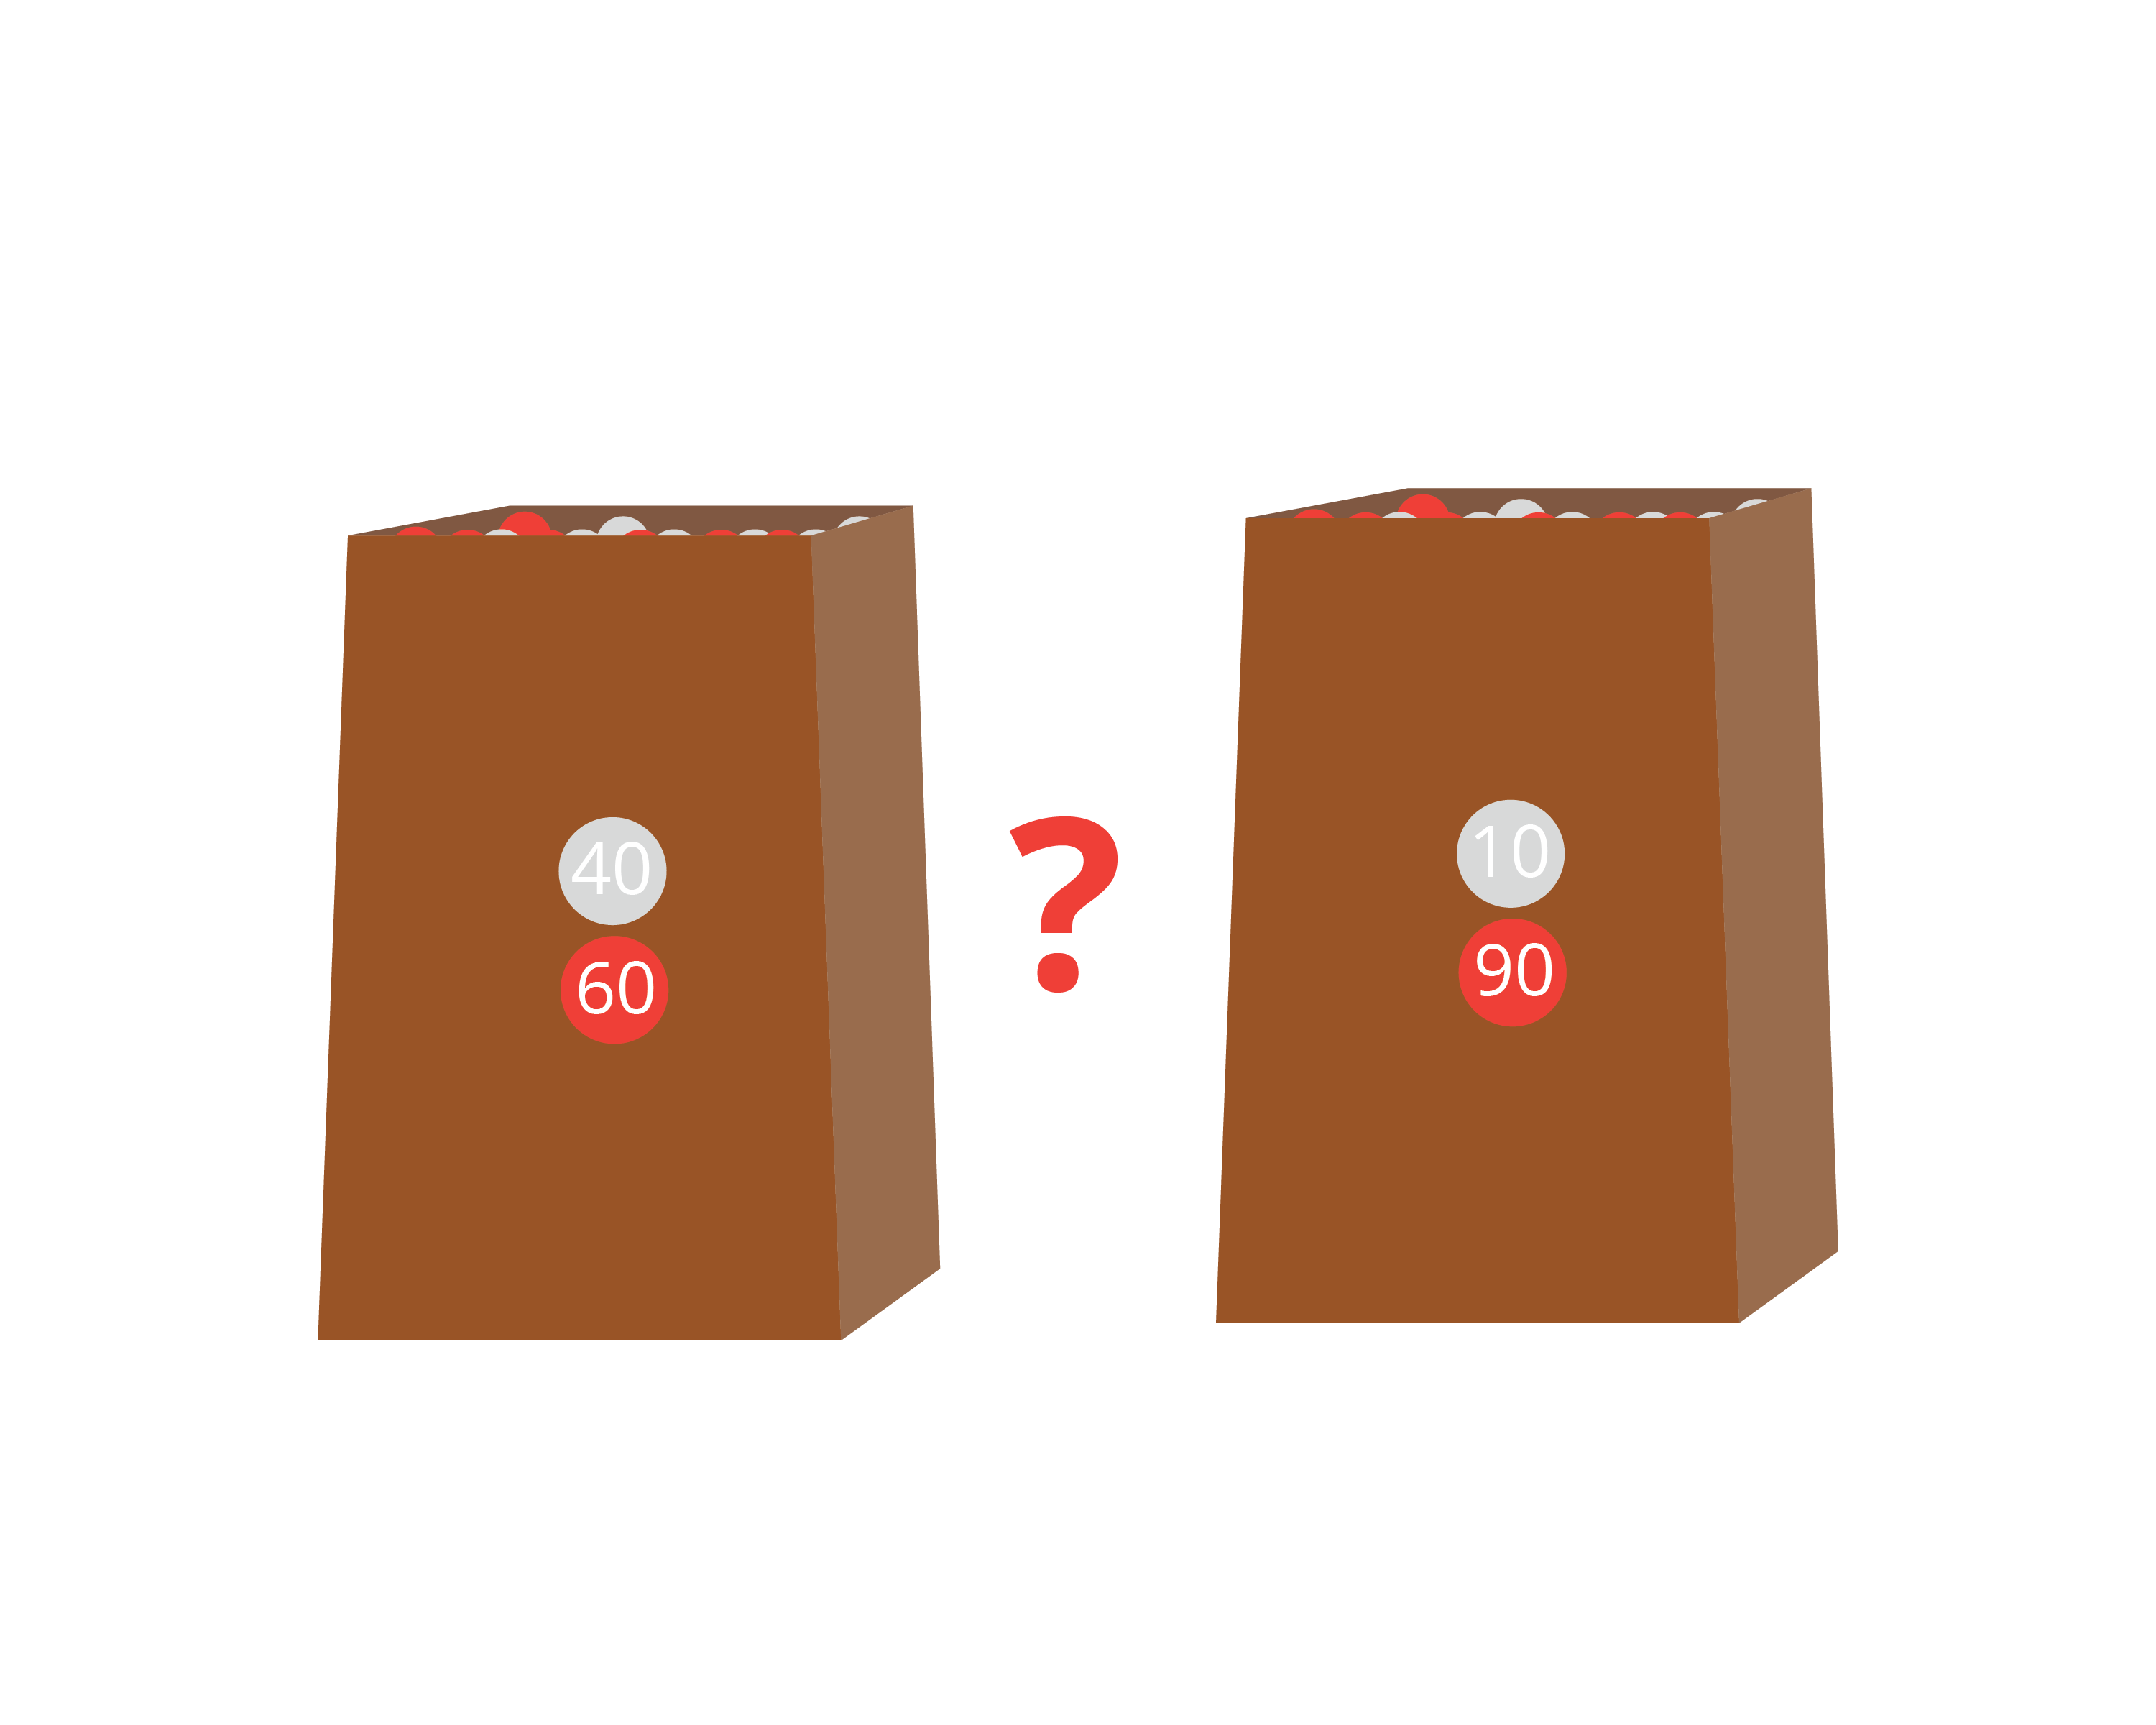
\includegraphics[width=0.8\textwidth]{bags.png}

Your friend says, ``Guess which bag is mostly red marbles.'' You pick one.

``What is the probability that this is the bag that is mostly red marbles?''
 You think to yourself "There is a 50 percent chance that this bag is mostly red marbles, and there is
also a 50 percent probability that it is the mostly-white-marbles bag.''

You then pick one marble from the bag: it is red. Now you must
update your beliefs. It is more likely that this is the
mostly-red-marbles bag. What is the probability now?

Bayes Theorem gives you the rule for updating your beliefs based on
new data.

\section{Bayes Theorem}

Let's say you have two events or conditions $C$ and $D$. $C$ is
``The person has a cough'' and $D$ is ``The person is waiting to see a doctor.''

Using the chain rule of probability, we now have two ways to calculate $p(C \text{ AND } D)$:
% ADD: add rule of probability to index

$$p(C \text{ AND } D) = p(C | D) p(D)$$

(The probability the person is at the doctor multiplied by the probability they have a cough if they are at the doctor.)

or 

$$p(C \text{ AND } D) = p(C | D) p(D)$$

(The probability the person has a cough multiplied by the probability they are at the doctor if they have a cough.) See Figure\ref{fig:bayes1}
% ADD: This needs a little more explanation
\begin{figure}[htbp]
    \centering
    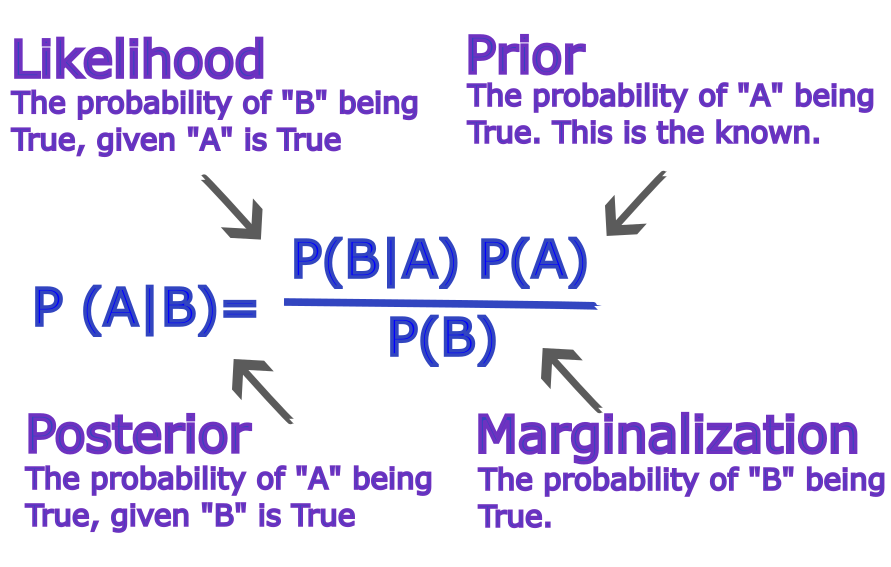
\includegraphics[width=0.8\textwidth]{Probability.png}
    \caption{A labelled figure of Bayes's Theorem Equation.}
    \label{fig:bayes1}
\end{figure}

Thus:
\index{bayes' theorem!formula}
$$p(D | C) = \frac {p(C | D)p(D)}{P(C)}$$

Now, you can calculate $p(D | C)$ (in this case, the probability that
you are waiting to see a doctor given that you have a cough.) if you
know:

\begin{itemize}
\item $p(C | D)$ (The probability that you have a cough given that you are waiting to see a doctor)
\item $p(D)$ (The probability that you are waiting for a doctor for any reason.)
\item $p(C)$ (The probability that you have a cough anywhere)
\end{itemize}

Pretty much all modern statistical methods (including most artificial
intelligence) are based on this formula, which is known as Bayes'
Theorem. It was written down by Thomas Bayes before he died in
1761. It was then found and published after his death.

\section{Using Bayes' Theorem}

Back to the example at the beginning. To review:

\begin{itemize}
\item There are two bags that look exactly the same.
\item Bag W has 60 white marbles and 40 red marbles.
\item Bag R has 10 white marbles and 90 red marbles.
\item You pull one marble from the selected bag: it is red.
\end{itemize}

What is the probability that the selected bag is Bag R? Intuitively,
you know that the probability is now more than 0.5. What is the exact
number?

In terms of conditional probability, we say we are looking for ``the probability
that the selected bag is Bag R, given that you drew a red marble'', or
$p(B_R | D_R)$, where $B_R$ is ``the selected bag is Bag R'' and $D_R$ is
``you drew a red marble from the selected bag''.

From Bayes' Theorem, we can write:

$$p(B_R | D_R) = \frac{ P(D_R | B_R) P(B_R) } {P(D_R)}$$

$P(D_R | B_R)$ is just the probability of drawing a red marble given that the
selected bag is Bag R. That is easy to calculate: There are 100
marbles in the bag, and 90 are red. Thus, $P(D_R | B_R) = 0.9$.

$P(B_R)$ is just the probability that you chose Bag R before you drew
out a marble. Both bags look the same, so $P(B_R)= 0.5$. This is
called \textit{the prior}, because it represents what you thought the
probability was before you got more information.

$P(D_R)$ is the probability of drawing a red marble. There was 0.5
probability that you put your hand into Bag W (in which 40 of the 100
marbles are red) and a 0.5 probability that you put your hand into Bag
R (in which 90 of the 100 marbles are red).  So

$$P(D_R) = 0.5 \frac{40}{100} + 0.5 \frac{90}{100} = 0.65$$

Putting it together:

$$p(B_R | D_R) = \frac{ P(D_R | B_R) P(B_R) } {P(D_R)} = \frac{(0.9)(0.5)}{0.65} = \frac{9}{13} \approx 0.69$$

Thus, given that you have pulled a red marble, there is about a 69\% chance
that you have selected the bag with 90 red marbles.

\section{Confidence}
\index{bayes' theorem!confidence}

Bayes' Theorem, then, is about updating your beliefs based on
evidence.  Before you drew out the red marble, you selected one bag
thinking it might contain 90 red marbles. How certain were you? 0.0 being complete disbelief and 1.0 entirely
confidence, you were 0.5. After pulling out the red marble, you were about 0.69
confident that you had chosen the bag with 90 red marbles.

The question ``How confident are you in your guess?'' is very
important in some situations. For example in medicine, diagnoses often
lead to risky interventions. Few diagnoses come with 100\% confidence.
All doctors should know how to use Bayes' Theorem. 
% ADD: This is why doctors are taught to think hourses not zebras

In a trial, a jury is asked to determine if the accused person is
guilty of a crime. Few jurors are ever 100\% certain. In some trials, Bayes'
Theorem is an exceptionally important tool.

%FIXME 
\section{The Monty Hall Problem}
\index{bayes' theorem!monty hall problem}

The Monty Hall Problem is a popular example in discrete probability and probability theory that highlights an application of Bayes' theorem. 

Here's the scenario\footnote{A few videos and a movie excerpt on this subject are linked in your digital resources.}
\begin{itemize}
    \item A contestant is presented with three doors. Behind one door is a brand new car; behind the other two doors are goats.
    \item The contestant selects one of the three doors, say Door A.
    \item The host, Monty Hall, who knows what is behind each door, then opens one of the remaining two doors, say Door B, revealing a goat.
    \item The contestant is then offered the choice to either stick with Door A or switch to the other remaining unopened Door B.
\end{itemize}

At first glance, many people assume that after Monty opens a door, there are two
doors left and hence the probability of winning the car is $1/2$ regardless of
whether one switches or stays. However, conditional probability and Bayes' Theorem reveal a different result.

Originally, the probability that you picked the right door, Door A, is $P(\text{A has the car}) = \frac{1}{3}$. 

Then, Monty Hall reveals Door B to contain a goat behind it. This changes things, as Door A remains a probability of $\frac{1}{3}$, while Door C, the unopened door, now contains the summed probability of the other two doors, $\frac{2}{3}$.

Proving this with Bayes' Theorem:

%FIXME simplify this
\begin{align*}
P(\text{Car behind C} \mid \text{Monty opens B}) 
&= \frac{P(\text{Monty opens B} \mid \text{Car behind C}) \, P(\text{Car behind C})}
         {P(\text{Monty opens B})} \\[6pt]
&= \frac{1 \cdot \tfrac{1}{3}}
         {\;P(\text{Monty opens B} \mid \text{Car behind A})P(\text{Car behind A}) 
         + P(\text{Monty opens B} \mid \text{Car behind B})P(\text{Car behind B}) 
         + P(\text{Monty opens B} \mid \text{Car behind C})P(\text{Car behind C})} \\[6pt]
&= \frac{\tfrac{1}{3}}
         {\;(\tfrac{1}{2})(\tfrac{1}{3}) + 0\cdot(\tfrac{1}{3}) + 1\cdot(\tfrac{1}{3})} \\[6pt]
&= \frac{\tfrac{1}{3}}{\tfrac{1}{6} + \tfrac{1}{3}} \\[6pt]
&= \frac{\tfrac{1}{3}}{\tfrac{1}{2}} \\[6pt]
&= \tfrac{2}{3}
\end{align*}

Thus, it is always in your interest to switch. If you ever have the luxury to be on a game show, make sure to use Bayes' Theorem before making your guesses. 
%%%%%%%%%%%%%%%%%%%%%%%%%%%%%%%%%
%% Bookfooter.tex by Aaron Hillegass
%% Nov 8, 2020

\appendix

\chapter{Answers to Exercises}
\shipoutAnswer

\bibliography{references}

\printindex

\end{document}